\chapter{A mecânica da penetração}

A balística terminal trata da última parte do processo balístico, na qual acontece o impacto entre o projétil e o anteparo. A palavra armadura será usada neste capítulo como referente à composição entre as camadas de proteção, de modo que ela se refere à composição, que pode contar com uma ou mais placas e estruturas de materiais diversos. O anteparo é a primeira camada, logo recebe o contato inicial. Existem duas classes gerais quando se fala em armadura, as passivas e as reativas. As reativas são aquelas nas quais a energia cinética do projétil é usada para disparar alguma medida de reação. O projétil pode, por exemplo, causar uma pequena explosão que gera uma onda na direção contrária ao deslocamento dele. A explosão pode destruí-lo ou mudar sua direção. \\

Neste capítulo o foco será em armaduras passivas. Nelas a energia do projétil não é usada e é função dos materiais presentes na armadura diminuí-la. O sistema desejável é leve e ao mesmo tempo resistente, porém este não é um feito simples. A simulação por elementos finitos usando algoritmos complexos de plasticidade, aplicados a casos envolvendo  deformações severas, são necessários para o estudo deste tipo de sistema. Muitas das conclusões clássicas advém da aplicação deste tipo de simulação. \\
Historicamente é dominante o uso de chapas maciças de aço na qual a armadura é o anteparo, não havendo uma composição com diferentes materiais e funções. O uso de chapas monolíticas de aço não apresenta problemas quanto à absorção de energia e constituem ótimas blindagens, quando as características mecânicas apropriadas estão presentes. Dentre as características m necessárias, a mais importante de acordo com \cite{Crouch} é a dureza, porém mesmo aços com dureza e microestrutura adequada necessitam de grandes espessuras quando expostos a um impacto em altas velocidades. \\

Um exemplo histórico disso é a tentativa de construção de um veículo chamado Panzerkampfwagen VIII Maus, pela Alemanha durante a segunda guerra mundial. Este veículo contaria com chapas de aço de 240 mm de espessura, todavia este tipo de chapa seja suficiente para absorver a energia de qualquer projétil da época. Sua fabricação devia ser extremamente dificultosa, \cite{Crouch} reporta que até hoje fazer uma chapa muito espessa ter as propriedades corretas ao longo de sua espessura é um desafio. O item crítico para a falha do projeto foi que nenhum sistema de motorização e transmissão da época conseguiria propelir suficientemente o veículo. Atravessa-lo por uma ponte também não seria possível por conta de sua enorme massa.  \\

 Em geral a absorção de energia e a massa possuem uma relação inversamente proporcional. Ao longo dos anos processos de fabricação avançados e novos materiais surgiram e se desenvolveram para aumentar a proteção oferecida por sistemas mais leves. Um grupo de materiais muito presente neste avanço é o de cerâmicos. Um dos grandes projetos nesta área foi patrocinado por uma organização americana chamada DARPA.\footnote{Darpa em inglês significa Defense Advanced Research Projects Agency, ou em português agência de projetos avançados de pesquisa em defesa} Este projeto, chamado programa de armaduras leves, fomentou a criação do primeiro modelo computacional para a simulação de armaduras cerâmicas. Este programa foi amplamente usado para gerar avanços no entendimento deste tipo de material, em situações de impacto balístico. Alguns relatórios originados destes estudos estão disponíveis de forma aberta, por exemplo \cite{firstreport}. Este capítulo busca revisar aspectos da mecânica da penetração que são pertinentes à armaduras compostas pela composição entre cerâmicas e metais. \\
 
  \section{O comportamento dinâmico}
 
 Em relação a taxas quasi-estáticas os materiais submetidos a altas taxas de deformação apresentam propriedades mecânicas diferentes. De acordo com \cite{Hazell} a resistência de forma geral costuma aumentar, metais tendem a ficar mais resistentes porém menos dúcteis, sem haver alteração na rigidez. O mecanismo deste tipo de alteração em metais pode ser explicado, de acordo com \cite{Hazell}, pelo impedimento da movimentação de discordâncias durante a deformação plástica.\\ 
 
 Tanto para cerâmicos quanto para metais a resistência é, na maioria dos casos, proporcional à taxa de deformação
 \begin{equation}
 	\boldsymbol{\sigma} \propto \dot{\boldsymbol{\varepsilon}}
 \end{equation}
 
onde $ \dot{\boldsymbol{\varepsilon}} $ é a taxa de deformação e sua unidade é $ s^{-1} $.\\
Durante uma deformação inelástica há severa transformação de trabalho em calor, logo a temperatura na região de deformação sobe vertiginosamente. Metais acabam por sofrer, em vários casos, redução da resistência por conta de altas temperaturas. Esta redução é mais difícil em materiais cerâmicos por conta de suas altas temperaturas de fusão, costumeiras neste tipo de material. Observe que isto se reflete nos modelos mais usados para cada material, que foram revisados no capítulo  \ref{Cap: ModConst}. O modelo mais usado em metais é o de Johnson-Cook e tem um termo que trata especificamente da sensibilidade da resistência à temperatura. Para cerâmicas, nos modelos mais usados, que sãos os de Johnson-Holmquist, não há menção direta à temperatura. \\ 

O processo de penetração pode ser classificado como adiabático por conta do pouco tempo para a dissipação do calor gerado. Como visto anteriormente, isto pode gerar zonas de enfraquecimento térmico severo em materiais suscetíveis, pois o calor fica concentrado em regiões pequenas. Outra variável termodinâmica que tem influência no processo é a pressão. Se antes os metais se prejudicavam com o aumento da temperatura agora as cerâmicas, em geral, são beneficiadas pelo aumento da pressão. Inclusive \cite{Hazell} cita que há grupos que sugerem que a pressão tem influência positiva maior sob a resistência ao escoamento do que a própria taxa de deformação.
Um ponto importante é o comportamento do material cerâmico pós falha, tanto \cite{Hazell} quando \cite{holmquist_johnson_2002} citam a dificuldade de mensurar a resistência do material pós falha. É conhecido que a pressão tem influência na resistência do material que falhou, \cite{holmquist_johnson_2002} discute brevemente tal ponto. Algumas técnicas de simulação avançadas permitem substituir o elemento que sofreu erosão por uma partícula livre fazendo com que a pressão não diminua no local, \cite{johnson_2011} comenta tais técnicas.\\

\section{Os modos de falha}

Quando se estuda a proteção é primordial conhecer o ofensor. Uma munição completa é apresentada na figura \ref{fig:projetilinteiro}. O funcionamento parte da explosão da espoleta (Primer), então o propulsor (Propellant) propele o projétil (Bullet).\\
\begin{figure}[H]
	\centering
	\caption{Munição de armas pequenas. (Para correção: Aqui tenho um problema com a nomenclatura. Traduzi small arms para armas pequenas, mas deve ter algum nome mais correto. E não traduzi a imagem pois não achei algo bem defindo, então preferi apresentar em inglês.)}
	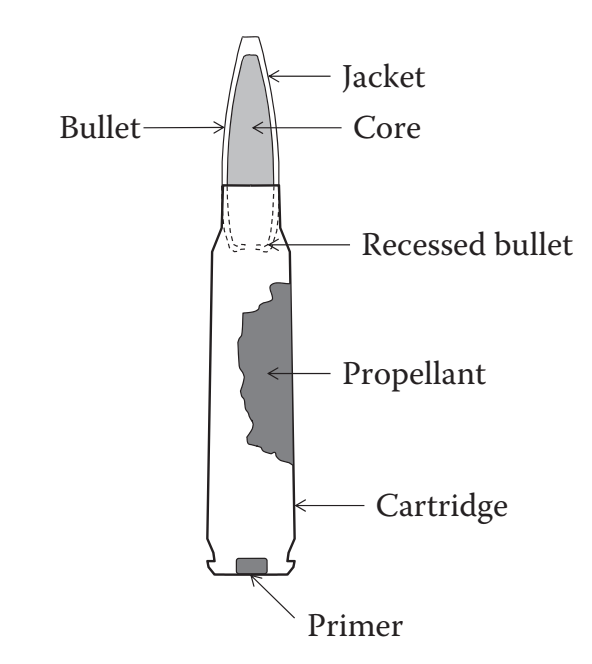
\includegraphics[width=0.5\linewidth]{images/projetil_inteiro.png}
	\label{fig:projetilinteiro}
	\fonte{\cite{Hazell}}
\end{figure}

Existem três grandes variáveis para o sucesso de um projetil, são elas sua velocidade de saída, seu material e sua geometria. O diâmetro destes projeteis aparece em milímetros ou em polegadas. Em milímetro as dimensões 7.62 e 5.56 são muito usadas, já em polegadas tem-se o .30 (7.62 milímetros)  e o .50 (12.7 milímetros) como exemplos. Ainda pertencendo a geometria o formato da ponta é de grande importância. As pontas esféricas são menos agressivas em relação às em ogiva ou cone.\\
Os materiais usados para a construção variam de acordo com a intenção do projetil. Os de menor poder penetrante são fabricados usando ligas de chumbo. Os de médio poder penetrante são fabricados de aço carbono ou aço carbono de baixa liga . Projeteis de alto poder de penetração são fabricados de um metal duro contendo carbeto de tungstênio em uma base de cobalto ou de ligas de aço altamente endurecíveis. A velocidade de saída pode variar muito entre os diferentes calibres, logo o limite considerado neste trabalho é na casa dos $ 2000 m/s $, baixo o suficiente para não haver ondas de choque em um metal ou cerâmica. \\


\subsection{A formação de orifício dúctil}
 O primeiro modo de penetração é a formação de um orifício dúctil, vide figura \ref{fig:buracoductil}. Ele é comum em placas dúcteis impactadas por projeteis pontiagudos. De acordo com \cite{Crouch} este mecanismo gera um furo de aspecto limpo e não retira massa do anteparo. O projetil age como um penetrador comparável à ponta de um durômetro quando este faz uma medição com sucesso, não havendo arredondamento de sua ponta. o ápice do projétil expulsa o material do anteparo para os lados de forma radial. A medida que o projetil avança há necessidade de abrir espaço para as secções que estão logo atrás do ápice. Este espaço é aberto pela deformação contínua do material do anteparo em maioria na direção radial e em minoria para outras direções normais à superfície do projétil. A maior parte destas deformações ocorre sob regime plástico, sendo assim a resistência dinâmica às tensões compressivas, em regime plástico, controlam a eficácia do material que falha desta forma. De acordo com \cite{Crouch} este é o modo de falha que traz a maior resistência a penetração enquanto apresenta os menores efeitos na face traseira do anteparo.
 
 \begin{figure}[H]
 	\centering
 	\caption{Formação de orifício dúctil.}
 	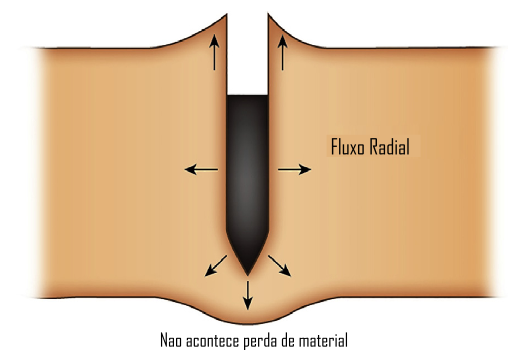
\includegraphics[width=0.5\linewidth]{images/Perfplast.png}
 	\label{fig:buracoductil}
 	\fonte{\cite{Crouch} traduzida pelo autor.}
 \end{figure}
 
 \subsection{O destacamento}
 
 O segundo modo é o "plugging" ou destacamento. Ele acontece, principalmente, quando o projétil apresenta ponta não aguda.  No momento subsequente ao contato entre projetil e anteparo há formação de um volume de partículas aceleradas que descrevem um cilindro na frente do projetil. As partículas localizadas fora deste volume não são aceleradas de forma significativa e é plausível considerar que permaneçam estacionárias em relação às do cilindro. Na área de fronteira entre as partículas aceleradas e não aceleradas ocorrem altas taxas de deformação cisalhante. De acordo com \cite{Crouch} já que o cisalhamento é extremamente localizado o material sofre pouca deformação plástica, logo sua absorção de energia é seriamente prejudicada. Existem materiais especificamente sensíveis a um tipo especial de destacamento que forma bandas finas de cisalhamento adiabático, nas quais o cisalhamento é ainda mais localizado fazendo com que a energia absorvida seja particularmente baixa. O nome dado a este fenômeno é cisalhamento adiabático e de acordo com \cite{Crouch} ainda não há um consenso sobre sua causa. O resultado do modo de falha destacamento é justamente o destacamento da porção de material logo a frente do projetil como visto na figura \ref{fig:furocilindro}. Este é um fenômeno considerado prejudicial em relação à absorção de energia, já que ocorre de forma localizada gastando pouca energia do projétil e  deve ser evitado. De acordo com \cite{Hazell} o destacamento ocorre com maior frequência quando a largura do anteparo e o diâmetro do projétil tem dimensão semelhante. Portanto como calibres mais comuns tem abaixo de $ 7.62mm $ chapas de $5$ a $ 8mm $ são as mais suscetíveis ao destacamento. Um ponto levantado por \cite{Crouch} é que o destacamento pode gerar um projetil secundário que deve ser contido. \\
 
   \begin{figure}[H]
 	\centering
 	\caption{Formação de um destacamento.}
 	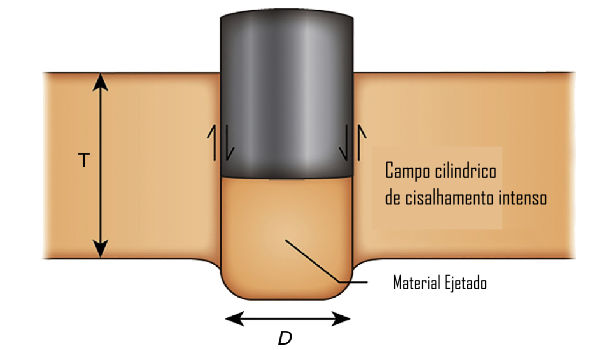
\includegraphics[width=0.5\linewidth]{images/plugging.png}
 	\label{fig:furocilindro}
 	\fonte{\cite{Crouch} traduzida pelo autor.}
 \end{figure}
 
 \subsection{A fratura conoidal e a cominuição}
 Este tipo de falha conjunta é encontrada em materiais duros como cerâmicos e vidros. \cite{Crouch} aponta que a fratura conoidal acontece em aços de ultra alta dureza, porém a cominuição não está presente. Na fratura conoidal a energia do projetil é transferida ao anteparo gerando trincas, chamadas hertzianas ou de hertz, que se propagam formando um cone adjacente à ponta do projetil, vide figura \ref{fig:hertz}. De acordo com \cite{Crouch} cones com maior ângulo são favoráveis ao desempenho balístico. O coeficiente de Poisson é a propriedade que mais tem mais influência sob este ângulo, maiores coeficientes de Poisson geram cones com ângulos maiores. \\
 
 A cominuição é caracterizada pela fratura do material formando várias partículas agudas de alta dureza, vide figura \ref{fig:cominuição}. A energia usada para o colapso do material não representa quantia significativa na redução da energia do projetil, porém a medida que este avança colide com as partículas formadas sendo erodido e perdendo massa. De acordo com \cite{neckel} a diminuição de massa ocorre até que as partículas do anteparo atinjam a velocidade do projetil  formando uma nuvem de partículas aceleradas. O processo de erosão descrito é responsável pela maior redução de energia em um anteparo de alta dureza que apresenta cominuição. Em algumas armaduras esta é a fonte principal de redução de energia do projetil, entretanto quando este tipo de falha está presente o sistema necessita de um material absorsor justaposto ao anteparo. Armaduras que usam anteparos cerâmicos normalmente possuem metais que são capazes de absorver tanto a energia residual do projetil quanto a energia da nuvem de partículas aceleradas pela colisão com o projetil.

 \begin{figure}[H]
 	\centering
 	\caption{Formação de trincas conoidais.}
 	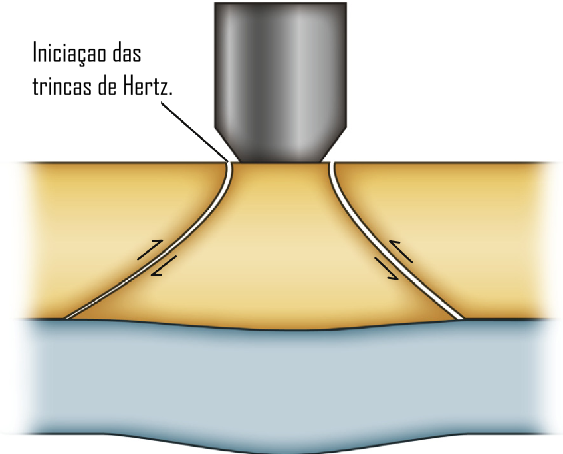
\includegraphics[width=0.5\linewidth]{images/hertz.png}
 	\label{fig:hertz}
 	\fonte{\cite{Crouch} traduzida pelo autor.}
 \end{figure}
 \begin{figure}[H]
 	\centering
 	\caption{Processo de cominuição.}
 	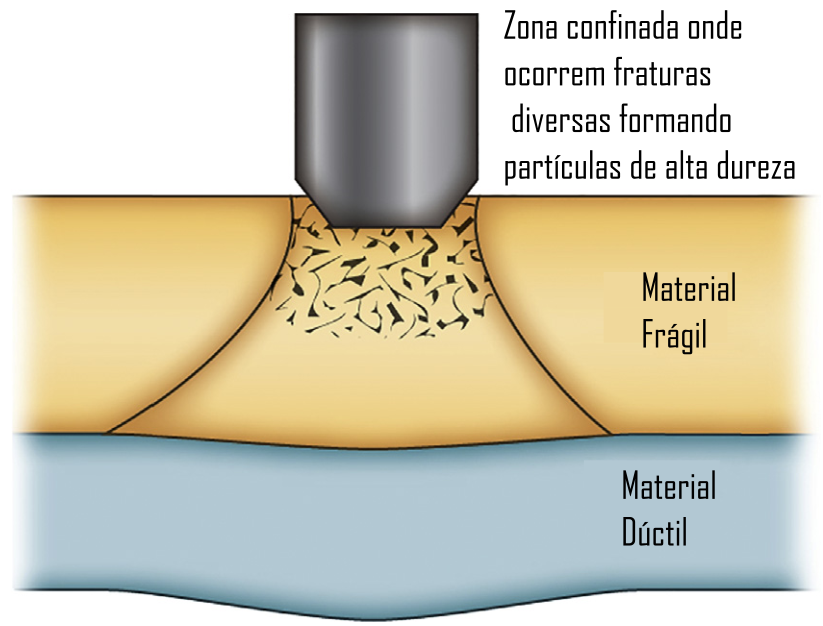
\includegraphics[width=0.5\linewidth]{images/comi.png}
 	\label{fig:cominuição}
 	\fonte{\cite{Crouch} traduzida pelo autor.}
 \end{figure}
 
 \section{As ondas de tensão}
 
 A formação de ondas de tensão acontece sempre que um objeto em movimento e um estacionário colidem. Em velocidades baixas as ondas de tensão são elásticas e aumentando a velocidade são formadas ondas de tensão plástica. Em velocidades muito  elevadas as ondas de choque são formadas, porém de forma geral tais velocidades estão fora do escopo deste trabalho.\\
 
 Quando solicitações quasi-estáticas são examinadas o ensaio de tração é feito para desenhar uma curva tensão vs deformação e este ensaio, quando feito de forma padrão, gera um estado uniaxial de tensão na peça. Uma curva tensão vs deformação em estado uniaxial de tensão é apresentada na figura \ref{fig:tensuniaxi}.
 
 \begin{figure}[H]
     \centering
     \caption{Curva tensão deformação em estado uniaxial de tensão.}
     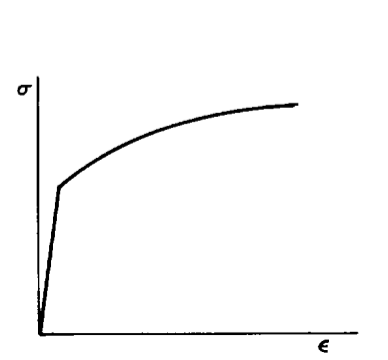
\includegraphics[width=0.5\linewidth]{images/tensuniaxial.png}
     \label{fig:tensuniaxi}
     \fonte{\cite{Zukas}}
 \end{figure}
 
 Porém quando o impacto em materiais é estudado o estado uniaxial de tensão não é mais conveniente, no sentido de que é difícil incitar tal estado em um impacto. O estado uniaxial de deformação é mais facilmente atingido, portanto este é o estado mais usado nestas situações. Este tipo de estado gera curvas como as da figura \ref{fig:defuniaxi}.
 
 \begin{figure}[H]
     \centering
     \caption{Curva tensão deformação em estado uniaxial de deformação.}
     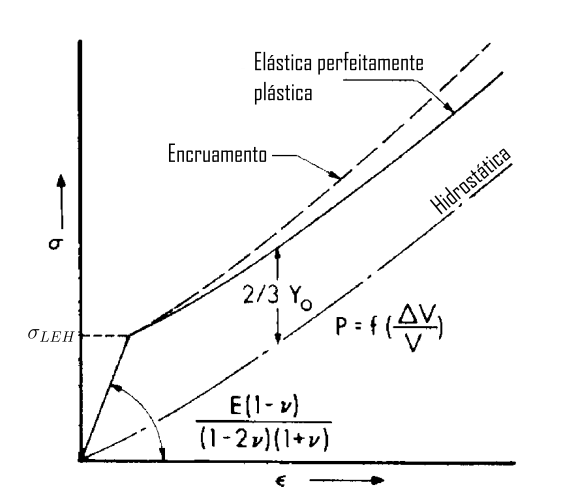
\includegraphics[width=0.5\linewidth]{images/defuniaxial.png}
     \label{fig:defuniaxi}
     \fonte{\cite{Zukas} traduzido pelo autor.}
 \end{figure}
 
 Veja que na figura \ref{fig:defuniaxi} também está presente o estado de tensões hidrostáticas. Com o acréscimo da tensão chegará um ponto onde a curva que considera a resistência do material será irrelevante numericamente. Este é o tipo de situação na qual os códigos de propagação de ondas foram criados, por isso o nome hidrocódigo surgiu. \\
 Na curva descrita pelo material estão representados dois cenários. Num o material apresenta comportamento perfeitamente plástico, noutro há encruamento. Veja que aqui o encruamento originalmente foi apresentado pelo autor \cite{Zukas} como originado apenas pela deformação, mas materiais cerâmicos tendem a apresentar aumento da resistência devido ao aumento da pressão também. \\
 
 Um ponto importante da curva é o limite elástico de Hugoniot ou $\sigma_{LEH} $. Ele marca a mudança de comportamento de elástico para plástico e é também a amplitude da onda elástica quando ondas plásticas estão presentes. Doravante onda elástica, onda plástica e onda de choque querem dizer onda de tensão elástica e por conseguinte. A velocidade da onda elástica é calculada usando a inclinação da reta em regime elástico seguindo a expressão
 
 \begin{equation} \label{eq:ondaelasticavel}
     c_{e} = \sqrt{\ddfrac{E(1- \nu )}{\rho_r (1 - 2\nu )(1+ \nu)}} 
 \end{equation}
 
 Caso as tensões forem superiores a \gls{hugoniot} a onda elástica se propagará com a velocidade descrita na equação \ref{eq:ondaelasticavel} e uma ou algumas ondas elásticas se propagarão de acordo com a seguinte equação
 
 \begin{equation} \label{eq:ondaplasticavel}
     c_{p} = \sqrt{\frac{1}{\rho} \frac{d \sigma}{d \varepsilon}}
 \end{equation}
 
 Portanto a velocidade de uma onda plástica está associada a derivada da tensão pela deformação no regime plástico. Quando o nível de deformação é muito alto esta derivada tende a ter valor muito elevado, aumentando muito a velocidade da onda em relação às anteriores. A imagem \ref{fig:elastochoque} mostra  o comportamento esperado de uma curva de tensão deformação em estado uniaxial de deformação até o estado de choque. \\
 
 
 \begin{figure} [H]
     \centering
     \caption{Gráfico dos regimes elástico, elastoplástico e de choque.}
     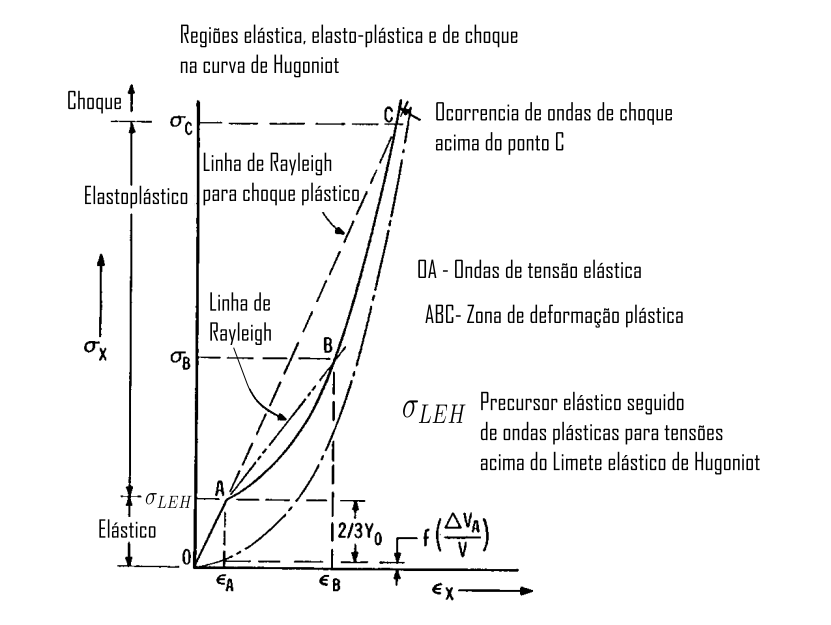
\includegraphics[width=0.5\linewidth]{images/elasticplasticshock.png}
     \label{fig:elastochoque}
     \fonte{\cite{Zukas} traduzido pelo autor.}
 \end{figure}
 
 O critério principal para o acontecimento de uma onda de choque é que a velocidade da onda plástica mais rápida seja suficiente para alcançar as ondas plásticas anteriores formando uma descontinuidade na curva que descreve a pressão ao longo do tempo, ou da distância, assim como é visto na figura \ref{fig:buildshock}. De acordo com \cite{Zukas} este tipo de acontecimento é esperado em impactos com velocidade superiores a $2000 m/s$, já \cite{Hazell} afirma que isto acontece quando a taxa de penetração do projetil é maior do que a velocidade do som no meio. A tabela \ref{tab:veldosom} mostra a velocidade do som em alguns meio comuns no âmbito da ciência balística. Veja que de acordo com \cite{Hazell} uma onda de choque se formaria apenas em velocidades muito altas em meios sólidos. Para armamentos pequenos tais velocidades são absurdas, porém \cite{Hazell} afirma que projeteis lançados por explosivos podem chegar aos $11000 m/s$.
 
  \begin{figure} [H]
     \centering
     \caption{Formação de uma onda de choque.}
     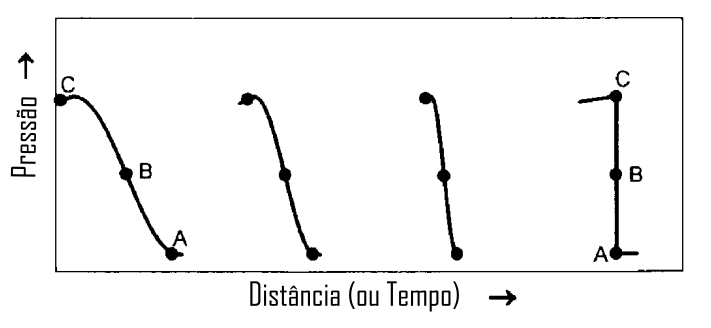
\includegraphics[width=0.5\linewidth]{images/buildshock.png}
     \label{fig:buildshock}
     \fonte{\cite{Zukas} traduzido pelo autor.}
 \end{figure}
 
 \begin{table}[H]
     \centering
     \caption{Velocidade do som em alguns materiais}
\begin{tabular}{|l|l|l}
\cline{1-2}
\textbf{Meio} & \textbf{Velocidade do som (m/s)} &  \\ \cline{1-2}
Ar            & 330                              &  \\ \cline{1-2}
Alumina       & 9900                             &  \\ \cline{1-2}
Alumínio      & 6300                             &  \\ \cline{1-2}
Aço carbono   & 5920                             &  \\ \cline{1-2}
Titânio       & 6100                             &  \\ \cline{1-2}
\end{tabular}
     \label{tab:veldosom}
     \fonte{\url{http://www.classltd.com/sound_velocity_table.html}}
 \end{table}
 
 
 \subsection{A impedância elástica.} (Talvez seja melhor retirar toda esta subseção. Pois ela chega em uma relação que apenas \cite{Hazell} cita como importante.)
 
 Quando duas placas estão em contato e uma delas sofre um impacto uma onda de tensão se propaga em direção à outra. Para manter a simplicidade, apenas ondas longitudinais serão consideradas. A onda original, chamada de incidente, é refletida e transmitida de acordo impedância elástica de cada material. A figura \ref{fig:ondasincierefle} apresenta  a direção de propagação das ondas longitudinais em questão. A tensão na interface estará em equilíbrio, de forma que
 
 \begin{equation} \label{eq:equitensao}
     \sigma_I + \sigma_R = \sigma_T
 \end{equation}
 
 onde  $ \sigma_I $ é a tensão incidente, $ \sigma_r $ a refletida e $ \sigma_T $ a transmitida. De acordo com \cite{Hazell} considera-se que não há espaços na interface e nem superposição de material. Por conta de tal consideração  as velocidades das partículas carregadas excitadas pelas ondas se comporta da seguinte maneira
 
 \begin{equation} \label{eq:equivel}
     u_{pI} + u_{pR} = u_{pT}
 \end{equation}
 
 Na qual $u_{p}$ significa velocidade da partícula e os  índices $I$, $R$ e $T$ mantém seu significado denotando incidente, refletido e transmitido. A velocidade da partícula pode ser calculada da seguinte maneira
 
 \begin{equation} \label{eq:calculodavel}
     u_p = \ddfrac{\sigma}{\sqrt{\rho_r E^{p/e}}}
 \end{equation}

Onde o símbolo $ E^{p/e} $ significa módulo de elasticidade ou o módulo elastoplastico. O módulo de elasticidade serve para situações elásticas e o elastoplastico para ondas plásticas.\\
 
 \begin{figure}[H]
     \centering
     \caption{Representação da reflexão e transmissão de ondas tensão.}
     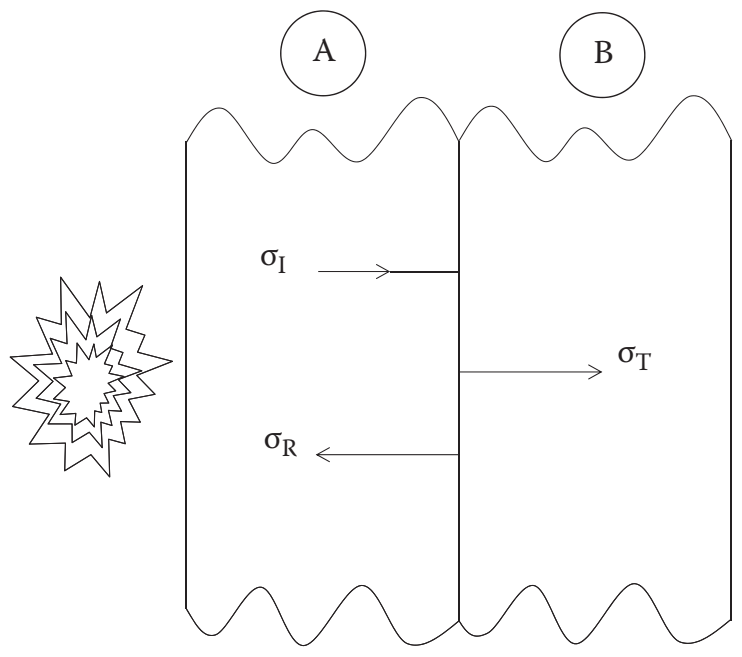
\includegraphics[width=0.5 \linewidth]{images/ondasincirefle.png}
     \label{fig:ondasincierefle}
     \fonte{\cite{Hazell}}
 \end{figure}
 
Considerando um impacto que não provocará inelasticidade. Ao aplicar \ref{eq:calculodavel} em \ref{eq:equivel} a seguinte expressão é obtida para dois materiais $A$  e  $B$ dispostos como na figura \ref{fig:ondasincierefle}.

\begin{align} \label{eq:velocitensao}
    u_{pI} = \ddfrac{\sigma_I}{\sqrt{E_A\rho_A}}, && u_{pR} = \ddfrac{-\sigma_R}{\sqrt{E_A\rho_A}}, && u_{pI} = \ddfrac{\sigma_T}{\sqrt{E_B\rho_B}}
\end{align}
 
  
 Agora resolvendo \ref{eq:velocitensao} e \ref{eq:equitensao} simultaneamente a seguinte expressão para a razão entre tensão refletida e transmitida é encontrada.
 
 \begin{equation}
     \ddfrac{\sigma_R}{\sigma_I} = \ddfrac{\sqrt{E_B \rho_B} - \sqrt{E_A \rho_A}}{\sqrt{E_B \rho_B} + \sqrt{E_A \rho_A}}
 \end{equation}
 
Usando esta relação, de acordo com \cite{Hazell} é possível otimizar o desempenho de materiais cerâmicos por meio de comparação entre dois metais de suporte diferentes. O melhor material para ser usado com a cerâmica é aquele que faz com que as tensões refletidas para sejam as menores possíveis. o cenário ótimo é aquele no qual a tensão refletida é compressiva. É importante apontar que o sinal das tensões é invertido na literatura balística, portanto tensões trativas tem sinal negativo. \\

Mesmo que as tensões refletidas sejam compressivas e portanto o acoplamento entre a cerâmica e o metal seja ótimo, ainda assim a cerâmica sofrerá fratura por conta das tensões trativas que são refletidas pela superfície livre da placa metálica. O ponto aqui é atrasar a fratura aumentando o desempenho da cerâmica quanto à penetração inicial.

\section{A aplicação de cerâmicas como classe de materiais de proteção.}

De acordo com \cite{Crouch} os cerâmicos são a classe de materiais mais importantes na blindagem moderna. Tanto óxidos quanto não óxidos tem importância elevada no meio, já que são ótimos disruptores de projéteis e portanto oferecem uma boa proteção ao impacto. Neste contexto estão inseridos os vidros, as cerâmicas transparentes e as translucidas, que desempenham funções outras, além da proteção balística. Este trabalho não abordará as cerâmicas transparentes, translucidas ou vidros. O foco aqui são cerâmicos opacos, cuja função é exclusivamente fornecer proteção.\\

A configuração padrão quando cerâmicas são usadas para proteção é a de dupla camada, sendo a primeira cerâmica e a segunda metálica. A função da cerâmica é erodir e fraturar o projetil reduzindo sua energia. De acordo com \cite{neckel_hotza_stainer_janssen_al-qureshi_2013} a cerâmica é responsável pela absorção de $85\%$ da energia na configuração usada por eles. \\

\subsection{Fatores importantes na aplicação de cerâmicas opacas.}

Mark Wilkins foi um dos grandes contribuidores para o entendimento da aplicação de cerâmicas em sistemas de blindagem. Sua série de relatórios, na qual o primeiro é \cite{firstreport}, aponta que a rigidez é de grande importância para o desempenho balístico em sistemas baseados no alumínio como placa de absorção. O modelo computacional de Wilkins foi um dos, senão o primeiro, a caracterizar fases importantes da penetração em materiais cerâmicos. \\

De acordo com \cite{reijel} é importante que a dureza da cerâmica seja superior à do projétil e \cite{Crouch} diz que é desejável que a razão dureza/densidade seja alta. Esta razão está ligada ao cone de fratura, já que quanto maior a base do cone melhor é o desempenho balístico. Quanto maior a espessura da cerâmica maior será a base do cone, então cerâmicas de menor densidade podem ser usadas em maior espessura, mantendo baixa a densidade de área. No âmbito de impacto balístico quando se diz densidade de área quer se dizer o resultado da densidade do material pela espessura da placa usada.  \\

\cite{Crouch} diz que não há consenso de um destacamento de propriedades medidas de forma estática que fazem com que o desempenho balístico aumente. Porém ele cita que as seguintes propriedades são importantes

\begin{itemize}
    \item Dureza : Sempre acima da dureza do projetil. Em geral acima de $10$ $GPa$
    \item Densidade: Deve ser a menor possível.
    \item Resistência em ensaio de flexão: Acima de $350$ $MPa$ é desejada.
\end{itemize}

Além disso \cite{kaufmann_cronin_worswick_pageau_beth_2003} discorre sobre a influência de algumas propriedades dos materiais cerâmicos em seu comportamento balístico usando experimentos com alumina $99.9 \%$ (CERAMOR), alumina modificada(CERAMOR-Z), carbeto de silício (Hexoloy) e carbeto de boro (Ceralloy
546). Tanto o carbeto de silício quanto o carbeto de boro são produtos comercias, já as aluminas não foram encontradas e o autor não cita a mudança realizada na alumina modificada. Porém os resultados são úteis mesmo sem o conhecimento da composição da alumina modificada. Os testes feitos por ele são de Profundidade de penetração em velocidades de $750$, $850$ e $910 m/s$ usando uma liga de alumínio $6061-T6$ como material de apoio.\\

As propriedades das cerâmicas testadas foram normalizadas usando a alumina $99.9\%$ como padrão, a figura \ref{fig:propceramis} apresenta estes resultados.    \footnote{A imagem apresentava qualidade muito baixa no artigo original, portanto foi necessário refaze-la, sem alteração qualquer nos dados apresentados, para o conforto do leitor deste texto.}

\begin{figure}
    \centering
    \caption{Propriedades das cerâmicas normalizadas pela alumina $ 99.9 \% $}
    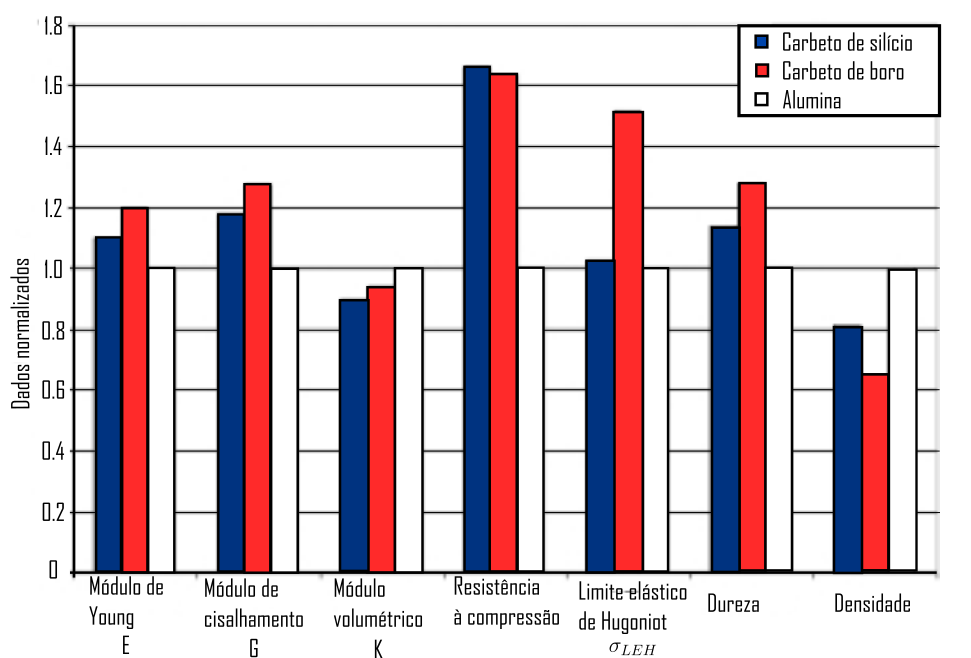
\includegraphics[width=0.8\linewidth]{images/propceramis.png}
    \label{fig:propceramis}
    \fonte{\cite{kaufmann_cronin_worswick_pageau_beth_2003} refeita e traduzida pelo autor.}
\end{figure}


Resistência à compressão: De acordo com \cite{shockey_marchand_skaggs_cort_burkett_parker_1990} ela é responsável pela resistência inicial da cerâmica a um projetil. No trabalho de \cite{kaufmann_cronin_worswick_pageau_beth_2003} foi observado que a resistência à compressão dos carbetos usados é semelhante e maior que a da alumina. O carbeto de silício apresenta melhores resultados em todos as velocidades usadas por \cite{kaufmann_cronin_worswick_pageau_beth_2003}, portanto ele conclui que ,devido aos dois carbetos apresentarem densidade de área semelhante, a resistência à compressão não é um fator dominante neste caso. Uma leitura diferente da feita pelo autor é que a resistência à compressão domina apenas a parte inicial da penetração e depois desta outras propriedades passam a dominar o evento. A motivação para tal é o resultado superior dos carbetos em relação à alumina. \\

Dureza: \cite{reijel} afirma que a dureza da cerâmica deve ser sempre maior que a do projetil e valores acima disto não são necessários. A importância da dureza está na erosão da ponta do projetil, dado que uma das partes iniciais do processo de penetração em uma cerâmica é justamente esta erosão. O processo de penetração na integra é revisado na seção seguinte.

Módulo de Young, de cisalhamento e volumétrico: O carbeto de boro tem o maior módulo de Young entre as cerâmicas testadas e portanto, dado que as densidades são semelhantes, possui a maior impedância elástica. Por ter maior impedância este deveria ter vantagem quanto ao desempenho balístico, pois as ondas refletidas seriam menos prejudiciais. Mesmo o carbeto de boro tendo uma vantagem esperada, o carbeto de silício apresentou resultados melhores em todos os testes. Quanto ao módulo de cisalhamento novamente o carbeto de boro tem o maior, porém  não desempenha os melhores resultados. O módulo volumétrico de todos as cerâmicas testadas são semelhantes. \cite{kaufmann_cronin_worswick_pageau_beth_2003} conclui que os módulos parecem não ter afetado os testes realizados por ele.

Limite elástico de Hugoniot: Aqui novamente o carbeto de boro é superior, porém é superado pelo carbeto de silício que tem  limite semelhante à alumina testada. \cite{kaufmann_cronin_worswick_pageau_beth_2003} conclui que o limite elástico de Hugoniot parece ter pouca influência na resistência de materiais cerâmicos ao impacto.

\subsection{Os mecanismos de absorção de energia e o modo de falha}

O processo de falha de uma cerâmica impactada por um projetil é apresentado passo a passo na figura \ref{fig:processo}.
\cite{Crouch} afirma que todas as fraturas relacionadas com as trincas de hertz e a cominuição são responsáveis pela diminuição de apenas $1\%$ da energia do impacto. Grande parte da energia do projetil é consumida através da erosão, portanto a cominuição é extremamente importante. De acordo com \cite{anderson} é uma das partes mais importantes do processo e é um dos fatores mais importantes na penetração. Outra indicação disto é trazida por \cite{holmquist_johnson_2002} que faz comparações da penetração entre um modelo que considera ou não a falha do material. Nas simulações onde o material não falha os valores previstos são irreais. Naquelas onde a porção do material abaixo do material falha gradativamente, de acordo com o modelo de Johnson-Holmquist, a penetração é corretamente prevista. De certa forma este é o caminho encontrado para simular a cominuição, já que seria muito complexo replicar o fenômeno em si. \\

De acordo com \cite{Crouch} é extremamente importante que todos os passos da figura \ref{fig:processo} ocorram na ordem descrita. A presença de porosidades nas adjacências do impacto é algo a ser evitado ao máximo, já que esta pode reduzir muito a resistência do cerâmico em compressão. \cite{Crouch} realizou experimentos de impactos em locais onde trincas originadas em impactos anteriores estavam presentes. Foi observado que houve redução de $9\%$ no desempenho balístico. 



\begin{figure}
    \centering
    \caption{Processo de penetração de um projetil em uma cerâmica suportada por um laminado.}
    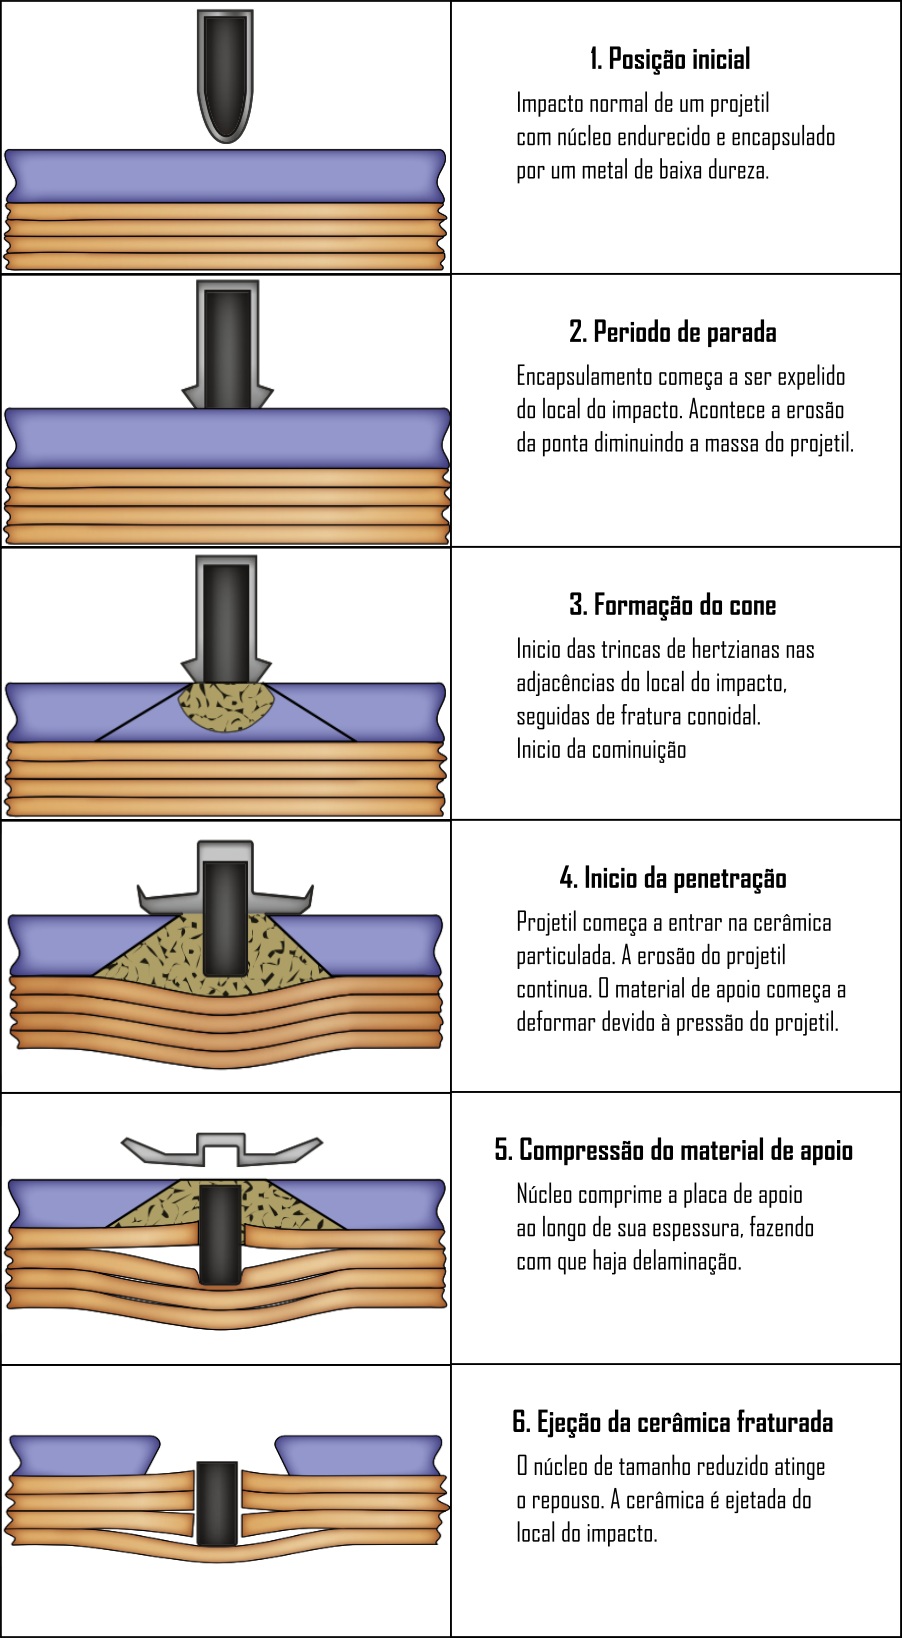
\includegraphics[width=0.7\linewidth]{images/processodepenetra.png}
    \label{fig:processo}
    \fonte{\cite{Crouch} traduzida pelo autor.}
\end{figure}


 